\chapter{Implementação}

\section{Força Propulsiva}

\par A propulsão por foguete é fundamentada na ejeção de um propelente com massa em alta velocidade, gerando força de acordo com a Terceira Lei de Newton.

\par A peça crucial em um motor foguete é o bocal, já que tem influência direta na produção da força propulsiva. A magnitude da força de tração é proporcional à vazão mássica oferecida pelo bocal, que, por sua vez, depende diretamente da área deste. A pressão estática do gás de exaustão ($p_e$) e a pressão atmosférica na saída do bocal ($p_a$) também afetam a força de tração produzida. Quando $p_e > p_a$, o bocal é categorizado como subexpandido, condição que ocorre em altas altitudes. Por outro lado, um bocal é superexpandido quando $p_e < p_a$. 

\par Um bocal de expansão completa é aquele em que $p_e = p_a$ (sem perdas de tração). Tais considerações podem ser verificadas pela equação de força propulsiva, que determina a força de tração resultante da ejeção do propelente através do bocal, seguindo a Segunda Lei de Newton aplicada a um corpo de massa variável:

\begin{equation}
\mathbf{f}_T=-\Delta m \frac{d\left(\mathbf{v}+\mathbf{v}_e\right)}{d t}-\mathbf{v}_e \frac{d \Delta m}{d t}-A\left(p_e-p_a\right) \frac{\mathbf{v}_e}{v_e}
\label{eq:prop}
\end{equation}

\par Na equação \ref{eq:prop}, $v$ é a velocidade do centro de massa do veículo, $v_e$ é a velocidade do gás de exaustão em relação ao centro de massa do veículo, $\Delta m$ é a massa instantânea do gás de exaustão, $A$ é a área de saída do bocal (normal a $v_e$), $p_e$ é a pressão estática do gás de exaustão e $p_a$ é a pressão atmosférica.

\section{Equação do Foguete}
\label{sectionfoguete}

\par Com os ideais passados no curso, foi obtida uma equação simplificada a qual foi denominada equação de foguete, vista em:

\begin{equation}
v-v_0=v_e \ln \frac{m_0}{m}
\label{eq:foguete}
\end{equation}

\par De acordo com a equação do foguete, a variação de velocidade é diretamente proporcional à velocidade de exaustão relativa, considerando uma redução específica na massa do veículo. Como a operação de um foguete geralmente ocorre em curtos intervalos de tempo, comparados ao período orbital, é plausível supor que a velocidade muda quase instantaneamente. Assim, consideramos que o motor do foguete fornece um impulso de velocidade $\Delta v = v - v_0$. Manipulando a equação do foguete, obtemos a seguinte relação:

\begin{equation}
v_e = -\frac{mdv}{dm}
\end{equation}

\par Esta equação indica que a velocidade de exaustão é igual à alteração na quantidade de movimento linear do foguete por unidade de massa de propelente consumida. O impulso específico é definido como a variação da quantidade de movimento linear por unidade de peso do propelente consumido e pode ser expresso como:

\begin{equation}
I_{sp} = \frac{v_e}{g}
\end{equation}

Com estas definições, a equação do foguete pode ser reescrita da seguinte forma:

\begin{equation}
\Delta v = I_{sp} g \ln \frac{m_0}{m}
\label{eq:foguetefinal}
\end{equation}

\subsection{Foguetes de um estágio}

\par A teoria do foguete de um estágio descreve como o foguete se comporta considerando suas principais componentes de massa: 

\begin{itemize}
    \item Massa de propelente ($m_p$);
    \item Massa de carga útil ($m_L$);
    \item Massa estrutural ($m_s$). 
\end{itemize}

\par Diante disso, a massa inicial e final do foguete são dadas, respectivamente, por:

\begin{equation}
m_0 = m_L + m_s + m_p   
\end{equation}

\begin{equation}
m_f = m_L + m_s  
\end{equation}

\par Duas razões-chave são importantes na teoria do foguete de um estágio: a razão estrutural $\sigma$ e a razão de carga útil $\lambda$.

\par A razão estrutural $\sigma$ é definida como a massa estrutural dividida pela soma da massa estrutural e da massa de propelente:

\begin{equation}
\sigma = \frac{m_s}{m_s + m_p}
\end{equation}

Enquanto isso, a razão de carga útil $\lambda$ é definida como a massa de carga útil dividida pela massa inicial do foguete:

\begin{equation}
\lambda = \frac{m_L}{m_0}
\end{equation}

Com estas definições, o impulso total de velocidade $\Delta v = v_f - v_0$, para um foguete de um estágio no espaço, onde a ação da gravidade pode ser desprezada ao longo da direção da velocidade, é dado por:

\begin{equation}
\Delta v = -v_e \ln (\sigma + (1 - \sigma)\lambda) 
\end{equation}

\subsection{Foguetes de múltiplos estágios}

\par Foguetes de múltiplos estágios são utilizados para superar as limitações de desempenho dos foguetes de um estágio. O foguete é composto pela junção de N segmentos, cada um possuindo seu próprio propelente e estrutura. A estrutura inclui motores, tanques, revestimentos, elementos estruturais, sistemas embarcados, etc.

\parAs massas estruturais e de propelente de cada segmento são denotadas por $m_{s_k}$ e $m_{p_k}$, respectivamente, onde k = 1, 2, . . . N. A massa de carga útil $m_L$ está acoplada ao último segmento.

\par A massa total do foguete é a soma das massas de todos os segmentos e da carga útil:

\begin{equation}
m_0 = m_L + \sum_{k=1}^{N} m_{s_k} + m_{p_k}
\end{equation}

\par Razões de carga útil intermediárias são definidas para cada estágio. Cada estágio terá uma razão de carga útil associada, definida de modo que a massa $m_{0_{k+1}}$ seja a carga útil do estágio anterior k. Em outras palavras, o foguete do segmento k tem a função de deslocar toda a carga acima do mesmo, que consiste na própria carga útil mais a estrutura e o propelente dos estágios superiores. Assim, a razão de carga útil do estágio k é:

\begin{equation}
\lambda_k = \frac{m_{0_{k+1}}}{m_{0_k}}
\end{equation}

E a carga útil intermediária total é:

\begin{equation}
\lambda_T = \prod_{k=1}^{N} \lambda_k
\end{equation}

A razão estrutural do estágio k é definida como:

\begin{equation}
\sigma_k = \frac{m_{s_k}}{m_{s_k} + m_{p_k}}
\end{equation}

\par Além disso, cada estágio tem uma velocidade de exaustão associada, $v_{e_k}$. Deste modo, a equação do foguete para N estágios em série é dada por:

\begin{equation}
\Delta v = -\sum_{k=1}^{N} v_{e_k} \ln \left(\sigma_k + (1 - \sigma_k) \lambda_k\right)
\end{equation}

\par Essa equação representa a soma das contribuições de cada estágio para a velocidade total do foguete. A velocidade de exaustão $v_{e_k}$ e as razões de carga útil $\lambda_k$ e estrutural $\sigma_k$ de cada estágio k são fatores críticos para o desempenho do foguete de múltiplos estágios.

\subsubsection{Estágios em paralelo}

\par Quando os propulsores paralelos (\textit{boosters}) e o primeiro estágio do núcleo do veículo queimam simultaneamente, eles são agrupados e chamados de "estágio zero". Após a separação dos propulsores, o propelente restante no primeiro estágio do núcleo do veículo define o primeiro estágio do foguete. A força de propulsão do estágio zero é expressa pela seguinte equação:

\begin{equation}
f_{T0} = -v_{eb}\frac{dm_b}{dt} - v_{e1}\frac{dm_1}{dt} = -v_{e0}\frac{dm_0}{dt}
\end{equation}

\par Onde os subscritos $b$ e $1$ referem-se às quantidades relativas aos propulsores paralelos e ao primeiro estágio do núcleo do veículo, respectivamente. $v_{e0}$ e $m_0$ representam a velocidade média de exaustão e a massa total, respectivamente, do estágio zero do foguete.

\par Os propulsores queimam uma massa total de propelente, $m_{pb}$, possuindo uma massa estrutural $m_{sb}$. Portanto, as razões estruturais e de carga útil equivalentes a um foguete de estágio são:

\begin{equation}
\sigma_0 = \frac{m_{sb} + m_{s1}}{m_{sb} + m_{s1} + m_{pb} + m_{p1_0}}
\end{equation}

\begin{equation}
\lambda_0 = \frac{m_{0_1} - m_{p_{1_0}}}{m_{0_0}}
\end{equation}

Onde $m_{0_0} = m_{0_1} + m_{sb} + m_{pb}$ é a massa inicial antes da queima do estágio zero.

\par As razões equivalentes para o primeiro estágio são:

\begin{equation}
\sigma_1 = \frac{m_{s1}}{m_{s1} + m_{p1} - m_{p_{10}}}
\end{equation}

\begin{equation}
\lambda_1 = \frac{m_{0_2}}{m_{0_1} - m_{p_{10}}}
\end{equation}

Por fim, para o caso de múltiplos estágios em paralelo, a equação do foguete pode ser expressa como:

\begin{equation}
\Delta v = -\sum_{k=0}^{N} v_{e_k} \ln\left(\sigma_k + (1 - \sigma_k)\lambda_k\right)
\end{equation}






%%%%%%%%%%%%% AULA 21 INICIO
\section{Forças atuantes sobre o veículo espacial}

\subsection{Segunda Lei de Newton para corpos de massa variável}
A segunda Lei de Newton para corpos de massa variável é dada por:

\begin{equation}
    \sum_{f} + f_{T} = (m - \DELTA m)\frac{dv_{0}'}{dt}
\end{equation}

Na qual $(m - \DELTA m)$ representa a massa variável, enquanto $v_{0}'$ é a velocidade do CM do corpo de massa variável após a ejeção da massa, sendo que o somatório de forças externas também leva em conta a força sofrida pela massa ejetada. 

\subsection{Sistema de referência do Vento}

O sistema referencial do vento é definido com respeito à velocidade aerodinâmica, mas para esse curso, a atmosfera é estacionária e sem vento, então o vetor velocidade relativa é igual ao vetor velocidade aerodinâmica, então este é usado como base para as definições. Uma das forças atuantes é a força aerodinâmica, que é escrita nesse referencial. O sistema referencial do vento com respeito ao LVLH é mostrado na figura \ref{fig:refvento}, na qual a origem $o$ é o CM do veículo, o eixo $x_{v}$ aponta na direção do vetor velocidade relativa \textbf{v}, o eixo $z_{v}$ é definido de modo que o plano $x_{v}z_{v}$ seja normal ao plano horizontal e o eixo $y_{v}$ é definido de modo a completar o sistema cartesiano ortogonal da mão direita, sendo paralelo ao plano horizontal local. 

\begin{figure}[h]
    \begin{center}
        \caption{SRV com respeito ao LVLH}
        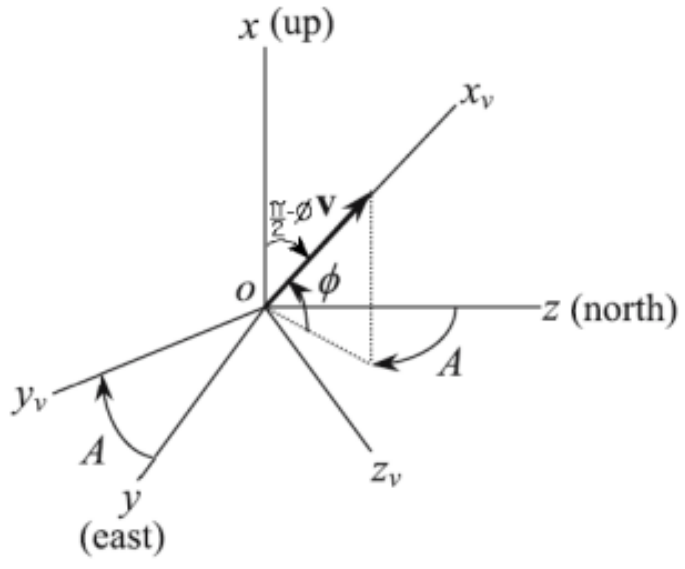
\includegraphics[width=1.5in]{figuras/vento.png}
        \label{fig:refvento}
        \fonte{\cite{livro:andre}}
     \end{center}
\end{figure}

A matriz de transformação do sistema LVLH para o SRV é definida pelo produto de matriz de rotação elementares:

\begin{equation}
C_{srv}^{lvlh} = 
 \left[\begin{array}{lll}
sin \phi & cos\phi sin A & cos\phi cos A \\
0 & cos A & -sinA \\
-cos \phi & sin \phi sin A & sin \phi cosA  
\end{array}\right]
\end{equation}

\subsection{Sistema referencial propulsivo}

O sistema de referência propulsivo é usado para definir o apontamento da força propulsiva com respeito ao SRV. A transformação do SRV para o SRP é encontrada a partir de uma sequência de rotações elementares:

\begin{equation}
C_{srp}^{srv} = 
 \left[\begin{array}{lll}
cos \mu cos \epsilon & sin \mu & -cos \mu sin \epsilon \\
-sin \mu cos \epsilon & cos \mi & sin \mu sin \epsilon \\
sin \epsilon & 0 & cos \epsilon  
\end{array}\right]
\end{equation}

\begin{figure}[h]
    \begin{center}
        \caption{SRP com respeito ao LVLH}
        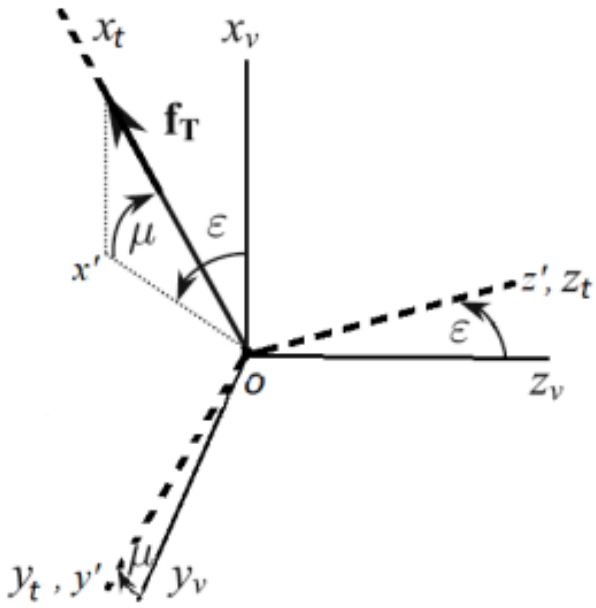
\includegraphics[width=1.5in]{figuras/srp.png}
        \label{fig:SRP}
        \fonte{\cite{livro:andre}}
     \end{center}
\end{figure}

 O SRP é mostrado na figura \ref{fig:SRP}, na qual a origem é o CM do veículo, o eixo $x_{t}$ aponta na direção da força propulsiva, o eixo $z_{t}$ está contido no plano $x_{v}z_{v}$ do SRV, e o eixo $y_{t}$ completa o sistema cartesiano ortogonal da mão direita. 

 \subsection{Força aerodinâmica}

 As forças aerodinâmicas escritas no SRV são dadas por:

 \begin{equation}
     f_{a_{srv}} = \left[\begin{array}{l}
-D \\
f_{y} \\
-L
\end{array}\right]
 \end{equation}

 A força de arrasto D têm sentido oposto à velocidade relativa, enquanto a força de sustentação L é perpendicular à força de arrasto, por fim, a força lateral é perpendicular ao vetor velocidade relativa. 

 \subsection{Força propulsiva}
 A força propulsiva que aponta ao longo do eixo $x_{t}$ com magnitude $f_{T}$ é escrita no SRP como:
\begin{equation}
     f_{T_{srp}} = \left[\begin{array}{l}
f_{T} \\
0 \\
0
\end{array}\right]
 \end{equation}

 No SRV, a força propulsiva é dada por:
\begin{equation}
     f_{T_{srv}} = \left[\begin{array}{l}
f_{T} cos \epsilon cos\mu\\
f_{T} sin\mu\\
-f_{T} cos \mu sin\epsilon
\end{array}\right]
 \end{equation}

Na qual os ângulos  $\mu$ e  $\epsilon$ são a angulação da tubeira em relação à velocidade relativa do veículo, que na prática são os ângulos do guimbal de 2 GDL responsáveis pela fatoração da tração. 

\subsection{Força gravitacional}

A força gravitacional é representada no referencial LVLH como:

\begin{equation}
     f_{g_{lvlh}} = m \left[\begin{array}{l}
-g_{c}\\
0\\
g_{\delta}
\end{array}\right]
 \end{equation}

Assim, a força gravitacional escrita no SRV é dada por:
\begin{equation}
     f_{g_{srv}} = m \left[\begin{array}{l}
-mg_{c}sin\phi + mg_{\delta}cos\phi cos A   \\
-mg\Delta sin A\\
mg_{c}cos\phi + mg_{\delta}sin\phi cos A  
\end{array}\right]
 \end{equation}

 \section{Dinâmica de translação}

 O modelo de mecânica de voo de translação do veículo possui seis equações diferenciais não lineares e três graus de liberdade, para os quais as variáveis de estado são as coordenadas esféricas da posição no referencial PCPF (distância radial $r$, longitude planetária $l$ e latitude $\delta$) e as coordenadas da velocidade relativa escritas no referencial LVLH (magnitude $v$, azimute da velocidade $A$ e elevação $\phi$). As equações são dadas por:


    
\begin{align}
\begin{split}
\dot{v} &= \frac{1}{m} (-D+f_{T}\cos \epsilon \cos\mu + mg_{c} \sin \phi + mg_{\delta} \cos A \cos \phi)\\
&\quad -r\omega_{e}^{2} \cos \delta (\cos A \sin \delta \cos \phi - \cos\delta \sin \phi)
\end{split}\\[1cm]
\begin{split}
\dot{A} &=  \frac{1}{mvcos\phi} (f_{y}+f_{T}\sin \mu - mg_{\delta} \sinA) - \frac{1}{vcos\phi} 2v\omega_{e} (\cosA\cos\delta \sin\phi - \sin\delta \cos\phi)\\
&\quad + \frac{1}{cosv\phi} (r\omega_{e}^{2} \sin A \sin \delta \cos \delta + \frac{v^{2}}{r} \sin A \tan\delta \cos^{2}\phi)
\end{split}\\[1cm]
\begin{split}
\dot{\phi} &= \frac{1}{mv}(L+f_{T} \cos \mu \sin\epsilon - mg_{c} \cos\phi - mg_{\delta}\cos A \sin \phi )\\
&\quad + \frac{1}{v}(2v\omega_{e} \sin A \cos\delta + \frac{v^{2}}{r} \cos \phi + r\omega_{e}^{2} \cos \delta (\cosA\sin\delta \sin\phi + \cos\delta \cos \phi))
\end{split}
\end{align}

%%%%%%%%%%%%% AULA 21 FIM 












































































%% Modelo Atmosferico aula 22

\section{Modelo Atmosférico}

Nesse contexto, vamos explorar os princípios de equilíbrio hidrostático e gás ideal para elaborar perfis verticais correspondentes à pressão, densidade e temperatura sob um estado estacionário de atmosfera padrão. Além disso, iremos estruturar uma variedade de parâmetros adimensionais essenciais para calcular as cargas aerodinâmicas e térmicas.

Ao descrever a atmosfera padrão, estabelecemos uma série de camadas sequenciais, que são caracterizadas pela variação do perfil de temperatura. Na Terra, as camadas são tradicionalmente designadas, em ordem crescente de altitude, como troposfera, estratosfera, mesosfera, termosfera e exosfera.

Algumas constantes termodinâmicas básicas são necessárias para configurar as camadas em equilíbrio termodinâmico. A equação que define a alteração linear da temperatura com a altitude em uma camada específica é:

\begin{equation}
T=T_{i}+a\left(h-h_{i}\right)
\end{equation}

Nessa equação, $i$ representa a camada em questão, $h$ é a altura geométrica e $a$ corresponde à taxa de lapso termal.

A taxa de lapso termal tem uma relação direta com o expoente politrópico $n$, que é crucial para avaliar a estabilidade do equilíbrio hidrostático em uma camada atmosférica. Conforme a seguinte equação, uma camada atmosférica é considerada termicamente estável se $a<0$ e instável se $a>0$.

\begin{equation}
a=-g \frac{1}{R} \frac{n-1}{n}
\end{equation}

Para valores de $a \neq 0$, a pressão como função da altitude geométrica nas camadas com variação linear de temperatura é definida como:

\begin{equation}
p=p_{i}\left(1+\frac{a\left(h-h_{i}\right)}{T_{i}}\right)^{-\frac{g_{0}}{R a}\left(1+\beta\left(\frac{T_{i}}{a}-h_{i}\right)\right)} \exp \left(\frac{g_{0} \beta}{R a}\left(h-h_{i}\right)\right)
\end{equation}

Nessa equação, $g_{0}$ denota a gravidade ao nível do mar, $R$ é a constante específica do gás e $\beta$ é definido por $\beta=2 / r_{0}$, onde $r_{0}$ é o raio médio da Terra.

No caso de camadas isotérmicas $(a=0)$, a pressão como função da altitude geométrica é expressa por:

\begin{equation}
p=p_{i} \exp \left(-\frac{g_{0}}{R T_{i}}\left(h-h_{i}\right)\left(1-\frac{\beta}{2}\left(h+h_{i}\right)\right)\right)
\end{equation}

Depois de calcular a temperatura e a pressão, podemos determinar a densidade utilizando a equação do gás ideal:

\begin{equation}
\rho=\frac{p}{R T}
\end{equation}

As expressões apresentadas são utilizadas para calcular a temperatura, a pressão e a densidade em qualquer altitude até $86 \mathrm{~km}$, faixa na qual a suposição de equilíbrio hidrostático ainda é válida.

Existem múltiplos padrões atmosféricos reconhecidos, com a taxa de variação da temperatura sendo um dos principais parâmetros usados como referência. No curso abordado, optou-se por um modelo misto, conforme proposto por Tewari (2007), que combina dois modelos distintos:

\begin{itemize}
\item No intervalo de $0 \leq h \leq 86 \mathrm{~km}$, aplica-se o padrão da atmosfera dos Estados Unidos de 1976. Este padrão contém duas camadas acima de $86 \mathrm{~km}$, que apresentam variação de temperatura não linear com a altitude e um certo grau de incerteza;

\item Para altitudes superiores a $86 \mathrm{~km}$, é usado o padrão atmosférico americano de 1962. Este padrão representa camadas até a altitude de $h=2000 \mathrm{~km}$, todas com temperatura variável linearmente. A combinação dos padrões atmosféricos dos Estados Unidos de 1976 e 1962 resulta em um modelo de 21 camadas (contando com as subcamadas). Esta combinação é ilustrada na figura abaixo.
\end{itemize}

\begin{figure}[h]
    \begin{center}
        \caption{Combinação de atmosfera padrão norte americana de 1976 e 1962}
        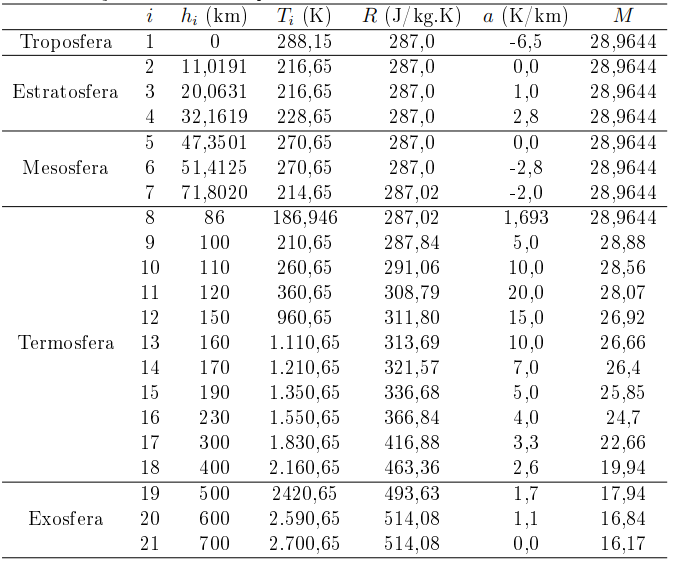
\includegraphics[width=3.5in]{figuras/atmos.png}
        \label{fig:atmos}
        \fonte{(TEWARI,2007), adaptado.}
     \end{center}
\end{figure}

Além das variáveis termodinâmicas básicas, alguns parâmetros adicionais podem ser calculados a partir do modelo atmosférico. Tais parâmetros são úteis para determinar cargas aerotérmicas:

\begin{enumerate}[(a)] 
\item Velocidade do som: 
\begin{equation}
a_{\infty}=\sqrt{\gamma R T}
\end{equation}
\end{enumerate}


\begin{enumerate}[(b)] 
\item Número de Mach:
\begin{equation}
M=\frac{v}{a_{\infty}}
\end{equation}
Onde $v$ representa a velocidade do veículo em relação à atmosfera.
\end{enumerate}

\begin{enumerate}[(c)] 
\item Coeficiente de viscosidade dinâmica:
\begin{equation}
\mu=1,458 \times 10^{-6} \frac{T^{\frac{3}{2}}}{T+110,4}
\end{equation}
\end{enumerate}

\begin{enumerate}[(d)] 
\item Número de Prandtl:
\begin{equation}
\operatorname{Pr}=\frac{\mu c_{p}}{k_{T}}
\end{equation}
Onde $k_{T}$ é o coeficiente de condutividade térmica do gás ideal, enquanto $c_{p}$ é seu calor específico a pressão constante, que pode ser calculado por:
\begin{equation}
c_{p}=\frac{R \gamma}{\gamma-1}
\end{equation}
\end{enumerate}

\begin{enumerate}[(e)] 
\item Número de Knudsen:
\begin{equation}
K n=\frac{\lambda}{l_{c}}
\end{equation}
Onde $\lambda$ é o caminho livre médio do fluxo não perturbado de moléculas e $l_{c}$ é um comprimento característico. O caminho livre médio é baseado no diâmetro de colisão $\sigma$, que pode ser calculado por:
\begin{equation}
\lambda=\frac{m}{\sqrt{2} \pi \sigma^{2} \rho N_{a}}
\end{equation}
Onde $m$ é a massa molecular em $\mathrm{kg} / \mathrm{Mol}$, e $N_{a}=6,0220978 \times 10^{23}$ é o número de Avogadro.
\end{enumerate}

\begin{enumerate}[(f)] 
  \item O parâmetro de regime de escoamento $d$, baseado no número de Knudsen:

  - Se $d=1$, o escoamento é livre molecular. Para $K n \geq 10$;

  - Se $d=2$, o escoamento é contínuo. Para $K n \leq 0,01$;

  - Quando $d=3$, o escoamento é de transição entre os dois regimes. Para $0,01<$ $K n<10$.
\end{enumerate}

\begin{enumerate}[(g)] 
\item Número de Reynolds:
\begin{equation}
R_e =\frac{\rho v l_{c}}{\mu}
\end{equation}
\end{enumerate}


\section{Modelo Gravitacional}

O modelo gravitacional utilizado é o mesmo utilizado no Trabalho 1, as principais hipóteses e pontos que devem ser reforçados são que um campo gravitacional conservativo, aplicado à segunda Lei de Newton para um corpo contínuo, permite a definição do potencial gravitacional:

\begin{equation}
g_i = \frac{\partial \phi_i}{\partial \mathbf{r}_{\mathbf{mi}}} = -Gm_i \frac{\mathbf{r}_{\mathbf{mi}}}{\left\|\mathbf{r}_{\mathbf{mi}}\right\|^3}
\end{equation}


Um modelo gravitacional para um corpo de simetria axial foi utilizado, levando em consideração o potencial gravitacional já descrito no Trabalho 1:

\begin{equation}
\Phi(r, \phi) = \frac{GM}{r}\left(1 - \sum_{n=2}^{\infty}\left(\frac{R_e}{r}\right)^n J_n P_n(\cos \phi)\right)
\end{equation}

Os polinômios de Legendre necessários para o cálculo do potencial são:

\begin{align}
P_2(v) &= \frac{1}{2}\left(3v^2 - 1\right) \\
P_3(v) &= \frac{1}{2}\left(5v^3 - 3v\right) \\
P_4(v) &= \frac{1}{8}\left(35v^4 - 30v^2 + 3\right)
\end{align}

Aplicando o gradiente à função potencial, é possível obter a aceleração da gravidade para coordenadas esféricas:

\begin{equation}
\frac{\partial \Phi}{\partial \mathbf{r}} = \frac{\partial \Phi}{\partial r} \mathbf{i}_r + \frac{\partial \Phi}{\partial \phi} \mathbf{i}_\phi + \frac{1}{r\sin \phi}\frac{\partial \Phi}{\partial \theta} \mathbf{i}_\theta
\end{equation}

\section{Modelo Aerodinâmico}

O modelo aerodinâmico desenvolvido abrange uma ampla faixa de regimes de escoamento, desde subsônico até hipersônico, levando em consideração a densidade do ar desde o meio contínuo até o livre molecular. Além disso, o modelo também incorpora diversos regimes de turbulência, bem como a dependência com a temperatura e reações químicas na termosfera e exosfera.

Em relação aos coeficientes de momento e força, geralmente são calculados três coeficientes de momento: rolagem ($C_{l}$), arfagem ($C_{m}$) e guinada ($C_{n}$); e três coeficientes de força: arrasto ($C_{D}$), sustentação ($C_{L}$) e lateral ($C_{Y}$). No entanto, neste contexto específico, apenas o movimento de translação do foguete é considerado, portanto, os coeficientes de momento não serão modelados. Os coeficientes de força serão avaliados de acordo com as seguintes hipóteses:

\begin{itemize}
    \item Foguetes são otimizados para baixa razão estrutural, o que implica que eles suportam baixos fatores de carga normais ou laterais. Portanto, voam com baixo ângulo de ataque e derrapagem, resultando em forças de sustentação e lateral muito pequenas, as quais podem ser consideradas nulas no modelo.
\end{itemize}

Dentro dessas limitações, apenas o coeficiente de arrasto será tratado. No voo de foguetes, o arrasto é importante para avaliar a perda de velocidade $\Delta v$ que o veículo sofre devido à resistência atmosférica.

Devido à complexidade em estimar modelos de arrasto, será adotado o modelo apresentado na referência (TEWARI, 2007), que é aplicável a uma cápsula de reentrada. No entanto, outros modelos também serão revisados a fim de fazer adaptações no modelo de referência.

Assumiremos que o veículo possui estabilidade estática, o que implica que os ângulos de ataque e derrapagem permaneçam nulos. Nesse caso, o coeficiente de arrasto da cápsula, para uma área de referência da base da cápsula de $S=4 \mathrm{~m}^{2}$, é dado por:

\begin{equation}
\left\{
\begin{array}{lr}
C_{D}=C_{D_{c}} & \text{se } K n<0,0146 \\
C_{D}=C_{D_{f m}} & \text{se } K n>14,5 \\
C_{D}=C_{D_{c}}+\left(C_{D_{f m}}-C_{D_{c}}\right)\left(\frac{1}{3} \log _{10} \frac{K n}{\sin 30^{\circ}}+0,5113\right) & \text{se } 0,0146 \leq K n \leq 14,5
\end{array}
\right.
\end{equation}

onde $K n$ é o número de Knudsen, calculado para o comprimento de referência $l_{c}=0,5 \mathrm{~m}$; $C_{D_{c}}$ é o coeficiente de arrasto no meio contínuo; e $C_{D_{f m}}$ é o coeficiente de arrasto no regime de escoamento livre molecular. O coeficiente $C_{D_{c}}$ é plotado como uma função do número de Mach, conforme ilustrado na Figura \ref{fig:aerodin}.

\begin{figure}[H]
    \begin{center}
        \caption{Coeficiente de arrasto contínuo em função do número de Mach}
        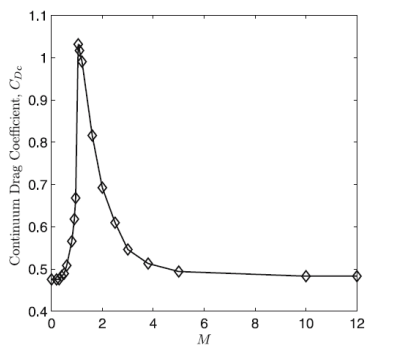
\includegraphics[width=3.5in]{figuras/mach.png}
        \label{fig:aerodin}
        \fonte{(TEWARI,2007).}
     \end{center}
\end{figure}

Podemos ver a partir da Figura \ref{fig:aerodin}, que o princípio de independência do número de Mach hipersônico é válido, tendo em vista que $C_{D_c}$ torna-se invariante com o número de Mach para $M > 8$.




\section{Voo ascendente de foguete}

A partir dos modelos desenvolvidos anteriormente, é possível simular o voo ascendente de um foguete, que possui duas aplicações de interesse: voo de sondagem e voo de inserção orbital.

No voo de sondagem, a trajetória é vertical ou quase vertical, com o objetivo principal de varrer uma faixa de altitude. Geralmente, a missão tem como objetivo adquirir dados em função da altitude ou realizar experimentos em microgravidade. Nesse tipo de trajetória, é necessário que o foguete mantenha uma trajetória vertical de forma estável, geralmente de maneira balística, sem a execução de manobras. Quando o veículo atinge a altitude máxima que atende aos objetivos da missão, a velocidade relativa se aproxima de zero ou se torna muito pequena.

Quanto ao voo de inserção orbital, também é lançado verticalmente ou próximo disso. No entanto, durante a ascensão, a trajetória deve curvar-se gradualmente, de modo que, no momento em que o motor do último estágio é desligado, o ângulo da trajetória seja próximo ou igual a zero. Ao atingir a altitude orbital e desligar o motor do último estágio, a velocidade relativa não será nula. Nesse momento, a velocidade do veículo deve ser igual à velocidade orbital desejada. Portanto, não basta apenas atingir a altitude desejada, mas também é necessário fornecer um impulso de velocidade compatível com a órbita naquela altitude.

A trajetória de inserção orbital pode envolver manobras ou ocorrer de forma puramente balística, dependendo do nível de precisão desejado, das características dos motores, da estabilidade e do controle. Independentemente da presença ou ausência de manobras, a trajetória deve garantir que o ângulo de trajetória seja próximo ou igual a zero no momento da inserção orbital, quando os motores são desligados.

Além das equações de movimento, do modelo aerodinâmico genérico, do modelo atmosférico e do modelo gravitacional mencionados anteriormente, é necessário especificar algumas características básicas do veículo:

\begin{itemize}
    \item Número de estágios;
    \item Massa de propelente de cada estágio;
    \item Massa estrutural de cada estágio;
    \item Massa da carga útil;
    \item Modelo propulsivo de cada estágio: tração e consumo de propelente;
    \item Parâmetros aerodinâmicos de cada estágio.
\end{itemize}

Se o foguete é de múltiplos estágios (N estágios), é necessário inserir na modelagem uma lógica de sequenciamento, a qual deve conter:

\begin{itemize}
    \item Tempo de ignição $t_{i_{k}}$ do estágio $k$, para $k = 1, \ldots, N$. Isso representa o momento em que o k-ésimo estágio é ligado.
   \item Tempo de queima $t_{q_{k}}$ do estágio $k$, para $k = 1, \ldots, N$. Isso representa o momento em que o k-ésimo estágio é desligado.
   \item Tempo de separação $t_{s_{k}}$ do estágio $k$, para $k = 1, \ldots, N$. Isso representa o momento em que o k-ésimo estágio é separado.
\end{itemize}

O sequenciamento de tempos da missão pode ser escrito de maneira relativa:

\begin{itemize}
    \item $t_{i_{k}} = t_{s_{k-1}} + T_{i_{k}}$, para $k = 2, \ldots, N$, onde $T_{i_{k}}$ é o tempo de espera para a ignição do estágio $k$ após a separação do estágio $k-1$.
    \item $t_{q_{k}} = t_{i_{k}} + T_{q_{k}}$, para $k = 1, \ldots, N$, onde $T_{q_{k}}$ é o tempo de duração da queima de propelente do motor do estágio $k$.
    \item $t_{s_{k}} = t_{q_{k}} + T_{s_{k}}$, para $k = 1, \ldots, N$, onde $T_{s_{k}}$ é o tempo de espera para a separação do estágio $k$ após a queima de seu propelente.

\end{itemize}


\subsection{Modelo Propulsivo}

Para o modelo propulsivo é necessário desenvolver os modelos de tração e variação de massa. Para um foguete com $N$ estágios, a variação de massa depende do desacoplamento dos estágios e do consumo de propelente pelos motores. Para os cálculos assumimos uma curva conhecida para a tração em função do tempo. Para determinar a massa em função do tempo, a partir da curva de tração fornecida, podemos utilizar a definição de impulso específico e a fórmula da tração reativa:

\begin{equation}
v_{e_{k}} = g I_{sp_{k}}, \quad f_{T_{k}}(t) = \dot{m}_{p_{k}} v_{e_{k}}
\end{equation}

Assumimos que a variação da tração devido à pressão no bocal de exaustão esteja modelada no impulso específico $I_{sp_{k}}$ ou na velocidade de exaustão $v_{e_{k}}$. Portanto, podemos determinar a relação entre $f_{T_{k}}(t)$ e $\dot{m}_{p_{k}}$ da seguinte forma:

\begin{equation}
\dot{m}_{p_{k}} = \frac{f_{T_{k}}(t)}{g I_{sp_{k}}}
\end{equation}

A vazão mássica de propelente $\dot{m}_{p_{k}}$ e a variação de massa do veículo $\dot{m}$ possuem sinais opostos, pois a vazão de propelente implica na diminuição da massa do veículo. Portanto, para calcular a taxa de variação da massa do veículo, trocamos o sinal de $\dot{m}_{p_{k}}$:

\begin{equation}
\dot{m} = -\frac{f_{T_{k}}(t)}{g I_{sp_{k}}}
\label{eq:252}
\end{equation}

Conhecendo a curva de tração em cada estágio durante a queima de propelente e a lógica de sequenciamento de estágios, o modelo da força propulsiva em função do tempo é dado por:

\begin{equation}
f_{T}(t) = 
\begin{cases}
f_{T_{k}}(t) & , \quad t_{i_{k}} \leq t \leq t_{q_{k}} \\
0 & , \quad t_{q_{k}} < t < t_{i_{k+1}}
\end{cases}
\end{equation}

Como o estágio $k+1$ não inicia sua queima instantaneamente após o estágio $k$, há um intervalo de tempo $\left(t_{q_{k}}, t_{i_{k+1}}\right)$ no qual nenhuma tração é aplicada. Esse intervalo tem duração $T_{s_{k}}+T_{i_{k+1}}$ e é chamado de fase de voo balístico. Em veículos lançadores de propulsão sólida e sem vetorização de tração, as únicas variáveis de controle são os tempos de duração das fases de voo balístico, ou seja, os intervalos de tempo $\left(t_{q_{k}}, t_{i_{k+1}}\right)$.

A lógica para determinação da massa, estágio após estágio, pode ser vista na equação condicional abaixo:

\begin{equation}
m(t) = 
\begin{cases}
m_{0_{1}} = m_{0} & , \quad t_{0} \leq t < t_{i_{1}} \\
m_{0_{k}} - \Delta m_{p_{k}}(t) & , \quad t_{i_{k}} \leq t \leq t_{q_{k}} \\
m_{0_{k}} - m_{p_{k}} & , \quad t_{q_{k}} < t < t_{s_{k}} \\
m_{0_{k+1}} = m_{0_{k}} - m_{p_{k}} - m_{s_{k}} & , \quad t_{s_{k}} \leq t < t_{i_{k+1}}
\label{eq:516}
\end{cases}
\end{equation}



A variável $\Delta m_{p_{k}}(t)$ na Equação \ref{eq:516} é definida como:

\begin{equation}
\Delta m_{p_{k}}(t) = \int_{t_{i_{k}}}^{t} \frac{f_{T_{k}}(\tau)}{g I_{sp_{k}}} d \tau
\end{equation}

No qual assumimos que:

\par - Toda a massa de propelente é consumida durante a queima de cada estágio;
\par - O desacoplamento de cada estágio é instantâneo.

\section{Algoritmos}

Todos os algoritmos desenvolvidos foram feitos de acordo com o fornecido pelo professor e adaptados de acordo com a necessidade do grupo. Os passos gerais do programa são:

\begin{itemize}
    
    \item Dados do veículo lançador e carga paga;

    \item Parâmetros de queima dos estágios;

    \item Parâmetros gerais do lançamento;

    \item Função que cálculo a dinâmica do movimento do veículo lançador;

    \item Funções auxiliares para os cálculos da dinâmica;

    \item Determinação dos parâmetros gerais da órbita;

    \item Plotagem dos gráficos.
    
\end{itemize}

Os programas elaborados para as aulas 19, 26 e 27 foram estruturados com uma função principal em um arquivo, complementada por diversas funções auxiliares dispostas em arquivos separados. No entanto, durante a criação dos códigos para a aula 29, que originalmente seguiam a mesma estrutura, enfrentamos inúmeros problemas relacionados à importação e declaração de variáveis globais, bem como aos inputs de funções.

Isso nos levou a adotar a estratégia de compilar todo o código em um único arquivo. Embora essa alteração tenha aumentado a demanda de processamento para a execução do código, ela permitiu solucionar os erros encontrados e efetivar a transposição do código do Matlab para Python.

É importante enfatizar que essa decisão foi tomada considerando o volume de erros encontrados e o prazo limitado que tínhamos à disposição. Apesar da demanda computacional adicional, consideramos essa medida necessária para cumprir o cronograma estabelecido.